% reducesymm/QFT/scfpo.tex , called by finiteQED.tex
% Predrag                               jul 10 2017

\section{Method of smooth conjugacies}
\label{sect:scfpo}

\begin{quote}
\emph{If Feynman knew Poincar\'e: How to replace many diagrams by one}

In quantum field theory the standard Feynman diagram methods become
quickly unwieldy at higher orders. However,
% as students of these notes will not be shocked to hear,
it is frequently observed that the sums of Feynman diagrams, each
individually complicated, simplify miraculously to rather compact
expressions.

Here comes a possible reason why that can be traced back to Poincar\'e,
and is perhaps not something that a field theorist would instinctively
hark to as a method of computing perturbative corrections: make the
dynamics linear (``free'') by flattening out the vicinity of a path
integral extremum by a smooth nonlinear coordinate transformation.
%This does not come cheap, but
The resulting perturbative expansion is more compact than the standard
Feynman diagram perturbation theory.
\end{quote}

\noindent
The smooth conjugacy method sketched here would require some serious work
to make it a workable quantum field theory scheme. The reader might
prefer to skip straight to the worldline formalism
\refsect{sect:worldline}.

The periodic orbit theory is a classical, deterministic
theory\rf{ChaosBook} that describes nonlinear systems in ``chaotic'' (for
low-dimensional systems) or ``turbulent'' (for PDEs) regimes. The theory
allows us to calculate long time averages in a chaotic system as
expansions in terms of the periodic orbits (cycles) of the system. The
simplest example (the deterministic analogue of the quantum evolution
operator) is provided by the {\FPoper}
\beq
\Lop \rho(x')=\int\!\!dx\,\delta(f(x)-x')\rho(x)
\ee{FPoper}
for a {\em deterministic} map $f(x)$ which maps a density distribution
$\rho(x)$ forward one integer step in time. The periodic orbit theory relates the spectrum
of this operator and its weighted evolution operator generalizations to
the periodic orbits via trace formulas, \dzeta s and spec\-tral
det\-er\-min\-ants\rf{GasAlo93,ChaosBook}.

For quantum mechanics the periodic orbit theory is exact on the
semiclassical level\rf{gutbook}, whereas the quintessentially quantum
effects such as creeping, tunneling and diffraction have to be included
as corrections. In particular, the higher order $\hbar$ corrections can
be computed perturbatively by means of Feynman diagrammatic
expansions\rf{GasAlo93}.
We illustrate how this works by the parallel, but simpler example of {\em
stochastic} dynamics.
Cvitanovi\'{c}\rf{chfield} {\em {Chaotic Field Theory}: {A} sketch}
% ~predrag/articles/hongkong/hk.tex
is a programmatic statement how this theory might connect to quantum
field theory, and, by a way of motivation, an easy introduction into
different approaches to incorporating stochastic corrections into
classical dynamics.

What motivated the work\rf{noisy_Fred,conjug_Fred,diag_Fred}
summarized in \refref{chfield} is the fact that the form of perturbative
corrections for the stochastic problem  is the same as for the quantum
problem, and still the actual calculations are sufficiently simple that
one can explore more orders in perturbation theory than would be possible
for a full-fledged quantum theory.
For the simple system studied, the result is a stochastic analog of the
Gutzwiller trace formula with  the ``$\hbar$ corrections'' computed to
five orders beyond what has been attainable in the quantum-mechanical
applications. Already a discrete time,
1-dimensional discrete Langevin equation\rf{vKampen92,LM94},
\begin{equation}
x_{n+1}=f(x_n)+\sigma\xi_n
\,,\label{Langevin}
\end{equation}
with $\xi_n$ independent normalized random variables, suffices to reveal
the structure of perturbative corrections.
We treat a chaotic system with weak external noise by replacing the
deterministic evolution $\delta$-function kernel of {\FPoper}
\refeq{FPoper} by $\Lnoise{}$,  the Fokker-Planck kernel corresponding to
\refeq{Langevin}, a peaked noise distribution function
\beq
\Lnoise{}(x',x) =\delta_\sigma(f(x)-x')
\,.
\ee{Lnoise}
In the weak noise limit the kernel is sharply peaked, so it
makes sense to expand it
in terms of the Dirac delta function and
its derivatives:
\beq
	\delta_\sigma(y)
	=
	\sum_{m=0}^{\infty} {a_m \sigma^m \over m!} \, \delta^{(m)}(y)
	=
	\delta(y) +
	a_2 {\sigma^2 \over 2} \delta^{(2)}(y) +
	a_3 {\sigma^3 \over 6} \delta^{(3)}(y) + \dots
	\,.
\label{delSigExp}
\eeq
where
\[
	\delta^{(k)}(y) = {\pde^k \over \pde y^k} \delta(y)
	\,,
\]
and the coefficients $a_m$ depend on the choice of the kernel.
We have omitted the $\delta^{(1)}(y)$ term in the above because
in our applications we shall impose
the saddle-point condition, that is,
we shift $x$ by a constant to ensure that the noise peak corresponds
to $y=0$, so $\delta_\sigma^{'}(0)=0$.
For example, if $\delta_\sigma(y)$ is a Gaussian kernel,
it can be expanded as
\bea
	\delta_\sigma(y)
	&=&
	{1 \over \sqrt{2 \pi \sigma^2}} e^{-{y^2/2\sigma^2} }
	=
	\sum_{n=0}^{\infty}
	\frac{\sigma^{2n}}{n!2^n} \delta^{(2n)}(y)
	\continue
	&=&
	\delta(y) + {\sigma^2 \over 2} \delta^{(2)}(y)
	 + {\sigma^4 \over 8} \delta^{(4)}(y) + \cdots
	\,.
\label{delGaussExp}
\eea




% clipped from ~predrag/WWW/talks/UChicago99.html
% Trace formulas for stochastic evolution operators
% Feb. 10, 1999
Analogies between noise and quantum mechanics
can be explored by casting stochastic dynamics into path integral form (a
stoch\-astic Wiener integral). The periodic orbit theory is a
nonperturbative, ``WKB''  method for approximating such integrals, which
can then be improved by systematic perturbative corrections. In the weak
noise case the standard perturbation theory is an expansion in terms of
Feynman diagrams. For semiclassical quantum mechanics of a classically
chaotic system such calculation was first carried out by
Gaspard\rf{GasAlo93}. The stochastic version, implemented by Dettmann
\etal\rf{noisy_Fred}, reveals features not so readily apparent in the
quantum calculation. Perhaps some of these could be of interest to
Kreimer and collaborators, \refsect{sect:HopfAlgebra}.

The Feynman
diagram method becomes quickly unwieldy at higher orders.%
$\footnotemark\footnotetext{
The matrix method, introduced by Vattay \etal\rf{diag_Fred},
based on Rugh's\rf{hhrugh92} explicit matrix
representation of the {\evOper} will not be
discussed here. If one is interested in evaluating
numerically many orders of perturbation theory and many eigenvalues, this
method is unsurpassed.
}$
% ~predrag/articles/noise/conjug/conjug.tex clipping
%	Carl &  Predrag				27 oct 1998
However, in the Feynman diagram approach pursued in \refref{noisy_Fred},
the authors observe that the sums of Feynman diagrams simplify
miraculously to rather compact expressions.

Now the surprise; one can compute the same corrections faster and to a
higher order in perturbation theory by integrating over the neighborhood
of a given saddlepoint \emph{exactly} by means of a nonlinear change of
field variables. This elegant idea of flattening the neighborhood of a
saddlepoint, introduced by Mainieri \etal\rf{conjug_Fred}, and referred
to here as the {\em smooth conjugation method}, is perhaps an altogether
new idea in field theory. The idea, that  can be traced back to
Poincar\'e\rf{poincare}, injects into field theory a method standard in
the construction of normal forms for bifurcations\rf{Katok95}: perform a
smooth nonlinear coordinate transformation
$x = h(y)$,
$ f(x) = h(g(h^{-1}(x)))$
that flattens out the vicinity of a fixed point and makes the map {\em
linear} in an open neighborhood,
$ f(x) \to g(y) = {\bf J} \cdot y$.
\vspace{2ex}
\\
\centerline{
 ${
	\raisebox{-4.0ex}[5.5ex][4.5ex]
		 {
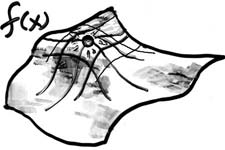
\includegraphics[height=10ex]{conjug-a}
		 }
        \atop
        \mbox{an arbitrary coordinatization}
        }$
~~~
$\Longrightarrow$
~~~
 ${
	\raisebox{-4.0ex}[5.5ex][4.5ex]
		 {
	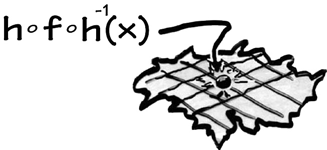
\includegraphics[height=10ex]{conjug-b}
		 }
        \atop
        \mbox{intrinsic, flat coordinates}
        }$
          }
\vspace{2ex}
\\
The resulting perturbative expansion turns out to be more compact than
the standard Feynman diagram perturbation theory; whether it is better
than the traditional loop expansions for computing field-theoretic
saddlepoint correction remains to be seen.

What is new is that the problem is being solved locally, periodic orbit
by periodic orbit, by translation to coordinates intrinsic to the
periodic orbit.

This local rectification of a map can be implemented only for isolated
non-degenerate fixed points (otherwise higher terms are required by the
normal form expansion around the point), and only in finite
neighborhoods, as the conjugating functions in general have finite radia
of convergence.

In this approach the neighborhood of each saddlepoint is rectified by an
appropriate nonlinear field transformation, with the focus shifted from
the dynamics in the original field variables to the properties of the
conjugacy transformation. The expressions thus obtained \emph{correspond
to sums} of Feynman diagrams, but are more compact.

We will try to explain this simplification in geometric terms that might
be applicable to more general field theoretic problems. The idea is this:
as the dynamics is nonlinear, why not search for a nonlinear field
transformation $\field = h(\tilde{\field})$ (a smooth conjugacy) that
makes the intrinsic coordinates as simple as possible? Schematically
--wrong in detail, but right in spirit-- find a smooth conjugacy such
that the action $S[\field] = S_0[\field] + S_I[\field]$ in the partition
function path integral becomes the free, quadratic action,
\beq
Z %[\source]
	 =  e^{W} %[\source]}
\,=\, \int [d\field] e^{S[\field]} % + \field \cdot \source}
\,=\, \int [d\tilde{\field}]
      \frac{1}{|\det \partial h(\tilde{\field})|^{1 \over 2}}
%      \, e^{\tilde{S}_0[\tilde{\field}]}
      \, e^{
      \frac{1}{2}
      \transp{\tilde{\field}}\frac{1}{\Delta}\tilde{\field}
            }
\,,
\label{Z-J}
\eeq
at the price of having the determinant of the
conjugacy Jacobian show up as a weight.

\refRef{noisy_Fred} treats the problem of computing the spectrum of this
operator by standard field-theoretic Feynman diagram expansions. Here we
formulate the perturbative expansion in terms of smooth conjugacies and
recursively evaluated derivatives. The procedure, which is relatively
easy to automatize, enables us to go one order further in the
perturbation theory, with much less computational effort than Feynman
diagrammatic expansions would require.

[TO BE CONTINUED]
